%
% -- Manlio Modugno

\documentclass{beamer} 
\usepackage{eulervm}
\usepackage{booktabs}
\usepackage{listings}
\usepackage{bold-extra}
\usepackage{cancel}
\usepackage{fancybox}
\usepackage{soul}
\usepackage[english]{babel}
\usepackage[utf8]{inputenc}
\usepackage{hyperref}
%\hypersetup{colorlinks=true,urlcolor=blue}

\newcommand{\codefont}{\fontsize{6}{8}\selectfont}
\lstset{language=[Sharp]C, 
captionpos=b, 
frame=lines,
lineskip= 2pt, %space between lines
basicstyle=\codefont, 
keywordstyle=\color{blue}, 
commentstyle=\color{green}, 
stringstyle=\color{red}, 
numbers=left, 
numberstyle=\tiny, 
stepnumber=2,
numbersep=5pt,
breaklines=true, 
breakatwhitespace=false,
showstringspaces=false,
frame=single,
tabsize=2,
emph={double,bool,int,unsigned,char,true,false,void},
emphstyle=\color{blue},
emph={Assert,Test},
emphstyle=\color{red},
emph={[2]\using,\#define,\#ifdef,\#endif},
emphstyle={[2]\color{blue}}
}

\mode<presentation>
\definecolor{title_color}{RGB}{2,128,181} 
\usetheme{Ilmenau}
\usecolortheme[named=title_color]{structure}
\setbeamercolor{palette quaternary}{use=structure,fg=black,bg=white} %header footer color
\useoutertheme[subsection=false]{smoothbars}
\setbeamercovered{transparent}
\setbeamertemplate{navigation symbols}{}
\setbeamerfont{subsection in toc}{size=\scriptsize}

\title{Studio\#start}
\author{Manlio Modugno}
\institute[GMTechnologies] 

\date[05.2016] 
{05.2016 - Presentazione piano di studio aziendale}

\subject{}

\graphicspath{{img/}}
\pgfdeclareimage[height=0.6cm]{mfg-logo}{img/mfgLogo}
\logo{\pgfuseimage{mfg-logo}}

%
% Content start
%
\begin{document}
\begin{frame}
  \titlepage
\end{frame}

\begin{frame}
  \frametitle{Argomenti Trattati}
  \tableofcontents
\end{frame}

\section{Corso}
\subsection{Obiettivi}
\begin{frame}
	\frametitle{Scopo - Obiettivi}	
	\begin{itemize}
  		\item<+-> Migliorare le nostre conoscenze
  		\item<+-> Avere piu' strumenti per affrontare le probematiche che si presentano
 		\item<+-> Evitare / ridurre compiti ripetitivi e noiosi
  		\item<+-> Automatizzare procedure manuali / controlli / etc. 
 		\item<+-> Essere piu' produttivi!
	\end{itemize}
\end{frame}

\subsection{Motivazioni}
\begin{frame}
	\frametitle{Motivazioni}	
	\begin{itemize}
  		\item<+-> Concetti applicabili anche a linguaggi non OO (i.e. bash / sql / os / etc..)
  		\item<+-> Le tecniche di programmazione istintiva (cut\&paste, code\&fix, ecc...) danno falsa sensazione di velocità...
 		\item<+-> .. che diminuisce progressivamente. Queste tecniche sono degenerative; raggiungono velocemente degli obiettivi nel breve periodo, ma degradano la qualità della base di codice, il che comporta un rallentamento durante l’implementazione delle funzionalità successive, fino al raggiungimento del collasso del codice
	\end{itemize}
\end{frame}

\begin{frame}
	\frametitle{Motivazioni(cont.)}	
	\begin{itemize}
  		\item<+-> Lo sviluppatore è anche progettista/designer
  		\item<+-> Il compilatore / interprete / etc. e' l'operario (traduce / esegue una specifica di alto livello)
 		\item<+-> Il design è un continuo che va dalla progettazione di alto livello o astratta fino a quella di di piu' basso livello (codice sorgente / script / sql / etc..)
	\end{itemize}
\end{frame}

\begin{frame}
	\frametitle{Motivazioni(cont.)}	
	\begin{center}
		\textbf{Il design del software è il codice}
	\end{center}
  	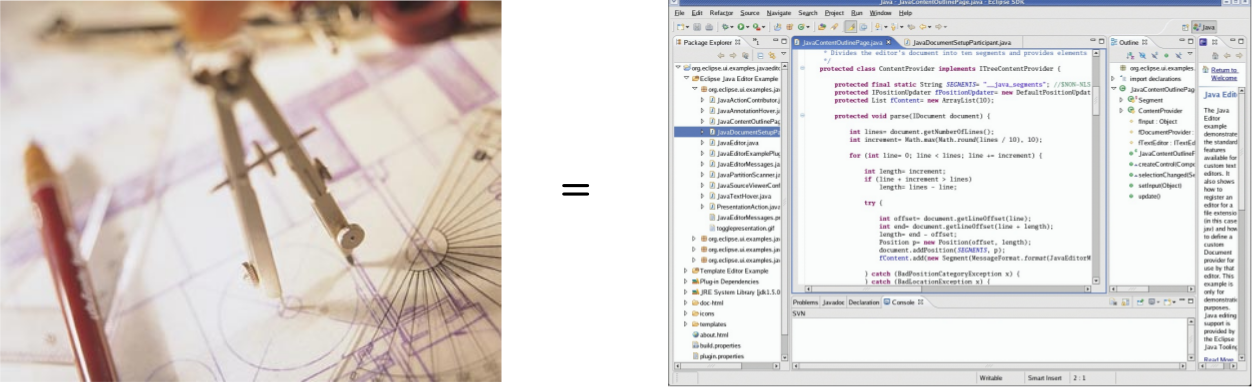
\includegraphics[scale=0.25]{equals}
\end{frame}

\subsection{Regole / Struttura}
\begin{frame}
	\frametitle{Regole / Struttura}
	\begin{enumerate}
  			\item<1-> Sessioni di studio individuale giornaliere (urgenze permettendo..) da 2 p su argomento scelto
  			\item<2-> Discussioni collettive con presentazione argomento a fine iterazione (1/2 settimane max.)
  			\item<3-> Presentatore casuale scelto all'inizio di ogni incontro collettivo
  			\item<4-> Ogni presentazione include uno o piu' esercizi legati all'argomento presentato. (Questo viene poi discusso / presentato all'inizio dell'incontro successivo)
	\end{enumerate}
%	\hfill
%	\vspace{0.05cm}
%	\pause
%	\begin{center}
%	\ovalbox{%
%		Gli utenti non concludono gli acquisti
%	}
%	\end{center}
\end{frame}

\subsection{Strumenti / Materiale}
\begin{frame}
	\frametitle{Strumenti}
	\begin{enumerate}
  			\item<+-> trello: board learning; carta con argomento scelto per Q/A,..
  			\item<+-> \LaTeX, Slide, mappe mentali, etc.. quello che si preferisce
  			\item<+-> Articoli, libri e riferimenti vengono messi sulla carta dell'argomento di studio
  			\item<+-> Ambiente di sviluppo!
	\end{enumerate}
\end{frame}

\section{Argomenti Core}
\subsection{Refactoring}
\begin{frame}
	\frametitle{Cosa vedremo: Refactoring}
	M.Fowler et al - Refactoring - Improving the Design of Existing Code (cap. 1 - 3) \\
	\textbf{Dipendenze:}
	\begin{itemize}
  			\item Class Diagram
  			\item Collaboration Diagram
  			\item Sequence Diagram
	\end{itemize}
	\textbf{Evil saga:}
	\begin{itemize}
  			\item Why extends is evil By Allen Holub
  			\item Why getter and setter methods are evil By Allen Holub
  			\item If is evil
	\end{itemize}
\end{frame}

\subsection{SOLID}
\begin{frame}
	\frametitle{Cosa vedremo: SOLID Principles}
	R. Martin - first five object-oriented design(OOD) principles \\
	\begin{itemize}
  			\item Single responsibility principle
  			\item Open/closed principle
  			\item Liskov substitution principle
  			\item Interface segregation principle
  			\item Dependency inversion principle
	\end{itemize}
\end{frame}

\subsection{GRASP}
\begin{frame}
	\frametitle{Cosa vedremo: Grasp Patterns}
	C. Larman - Applying UML and Patterns: An Introduction to Object-Oriented Analysis and Design and Iterative Development (General Responsibility Assignment Software Patterns) \\
	\begin{itemize}
  		\item Controller
		\item Creator
		\item High cohesion
		\item Indirection
		\item Information expert
		\item Low coupling
		\item Polymorphism
		\item Protected variations
		\item Pure fabrication
	\end{itemize}
\end{frame}

\section{Argomenti Next}
\subsection{Evoluzione}
\begin{frame}
	\frametitle{E poi..?}
	\begin{enumerate}
  			\item<+-> Una volta completato il ciclo core, cosa vedremo?
  			\item<+-> \textbf{The sky's the limit!}.. di imparare non si finisce mai..
  			\item<+-> GoF, articoli, studi piu' ``applicativi'' (particolare strumento/libreria/..), etc..
	\end{enumerate}
\end{frame}	

\section{Pericoli}
\subsection{New Toy Disease}
\begin{frame}
	\frametitle{Pericoli!}
	\begin{center}
		\textbf{New Toy Disease!}
	\end{center}
	\begin{center}
		\fbox{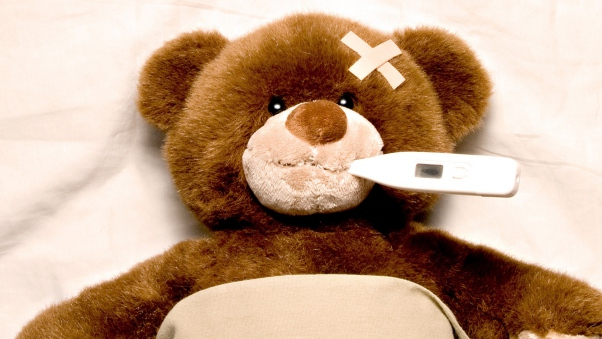
\includegraphics[scale=0.4]{toyDisease}}
	\end{center}
\end{frame}

\begin{frame}
	\frametitle{Pericoli!}
	\begin{center}
		\textbf{New Toy Disease!}
	\end{center}
	\begin{enumerate}
  		\item<1-> Wow!.. oggi ho imparato xyz.. che bello!
  		\item<2-> ..non vedo l'ora di usare xyz.. \textbf{devo} usarlo!
	\end{enumerate}
\end{frame}

\begin{frame}
	\frametitle{Pericoli!}
	\begin{center}
		\textbf{New Toy Disease! NO!}
	\end{center}
	\begin{enumerate}
  		\item Wow!.. oggi ho imparato xyz.. che bello!
  		\item \st{..non vedo l'ora di usare xyz.. \textbf{devo} usarlo!}
	\end{enumerate}
\end{frame}

\subsection{Taliban}
\begin{frame}
	\frametitle{Pericoli!}
	\begin{center}
		\textbf{Taliban!}
	\end{center}
	\begin{center}
		\fbox{
\includegraphics[scale=0.4]{taliban}}
	\end{center}
\end{frame}

\begin{frame}
	\frametitle{Pericoli!}
	\begin{center}
		\textbf{Taliban!}
	\end{center}
	\begin{enumerate}
  		\item<1-> Il ``sacro'' concetto xyz, scritto al versetto t della rota s, dice che non posso seguire la via del male..
  		\item<2-> ..quindi agiro' finchè la sacra interpretazione (mia) del divino sarà compiuta!
	\end{enumerate}
\end{frame}

\begin{frame}
	\frametitle{Pericoli!}
	\begin{center}
		\textbf{Taliban! NO!}
	\end{center}
	\begin{enumerate}
  		\item \st{Il ``sacro'' concetto xyz, scritto al versetto t della rota s, dice che non posso seguire la via del male..}
  		\item \st{..quindi agiro' finche' la sacra interpretazione (mia) del divino sara' compiuta}
  		\item Usiamo il buon senso..
	\end{enumerate}
\end{frame}

\subsection{Dining Philosophers}
\begin{frame}
	\frametitle{Pericoli!}
	\begin{center}
		\textbf{Dining Philosophers!}
	\end{center}
	\begin{center}
		\fbox{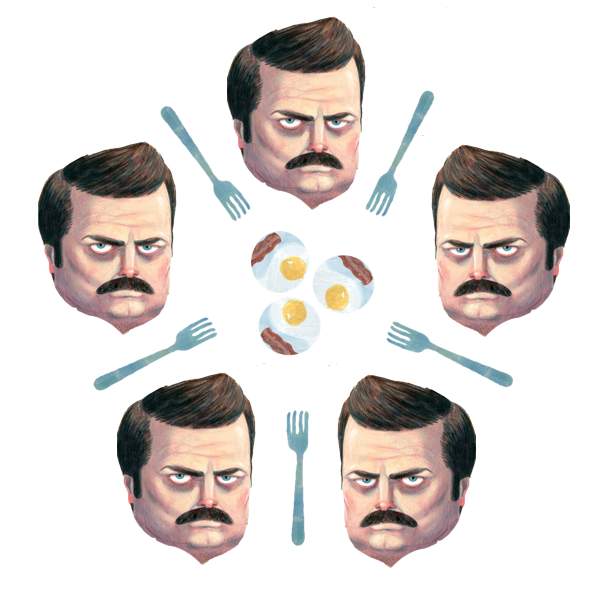
\includegraphics[scale=0.28]{dining}}
	\end{center}
\end{frame}

\begin{frame}
	\frametitle{Pericoli!}
	\begin{center}
		\textbf{Dining Philosophers!}
	\end{center}
	\begin{enumerate}
  		\item<1-> Evitiamo di intraprendere discussioni senza fine e inconcludenti..
  		\item<2-> Mettiamoci in discussione con mentalità aperta..
	\end{enumerate}
\end{frame}

\section{Next}
\subsection{Argomento}
\begin{frame}
	\frametitle{Argomento: Class / Collaboration Diagram}	

	\begin{itemize}
    		\item leggere \href{http://docs.oracle.com/javase/tutorial/java/concepts/object.html}{What Is an Object?}
     		\item leggere \href{http://docs.oracle.com/javase/tutorial/java/concepts/class.html}{What Is a Class?}
     		\item leggere (extra: first essay) \href{http://www.developerdotstar.com/mag/articles/PDF/DevDotStar_Reeves_CodeAsDesign.pdf}{What is software design?}
    		\item studiare \href{http://www.hristov.com/andrey/tu-sofia/uml/umlClassDiagrams.pdf}{class diagram 1}
    		\item studiare \href{http://www.ibm.com/developerworks/rational/library/content/RationalEdge/sep04/bell/index.html}{class diagram 2}
    		\item studiare \href{http://www.csee.wvu.edu/~ammar/rts/adv\%20rts/UML\%20tutorials/uml\%20diagrams/umlCollaborationDiagrams.pdf}{collaboration diagram}
	\end{itemize}
\end{frame}

\subsection{Esercitazione}
\begin{frame}
\frametitle{Esercitazione: Random Presenter}	

Realizzare (col linguaggio di programmazione che pare a voi) un'applicazione che ci permetta di selezionare il presentatore casuale delle sessioni collettive.

\textbf{Requisiti:}
\begin{itemize}
	\item Dev'essere usabile al momento della presentazione. Max 5 secondi.
	\item Deve permettere di escludere eventuali assenti. 
	\item (Se non lo avete già) create un account su github o su gitlab dove versionare il codice.
\end{itemize}
\end{frame}

\subsection{Enrollment}
\begin{frame}
	\frametitle{Enrollment}	
	Se l'idea vi piace...
	\begin{enumerate}
  		\item<+-> Aggiungetevi alla board 'learning' (visibilità di team, dovreste riuscire a trovarla..)
  		\item<+-> In alternativa mandatemi una mail
  		\item<+-> Cominciamo domani!
	\end{enumerate}
\end{frame}

\end{document}